\documentclass{article}
\usepackage{graphicx}
\usepackage[margin=1.5cm]{geometry}
\usepackage{amsmath}

\begin{document}

\title{Thursday Reading Assessment: DC Circuits and Error Propagation}
\author{Prof. Jordan C. Hanson}

\maketitle

\section{Memory Bank}

\begin{itemize}
\item $(x \pm \sigma_x) + (y \pm \sigma_y) = (x+y) + \sqrt{\sigma_x^2 + \sigma_y^2}$ ... Adding two averages with errors.
\item $V = i R$ ... Ohm's Law, with $V$ for voltage, $i$ for current, and $R$ for resistance.
\item $P = iV = i^2 R_{tot} = V^2/R_{tot}$ ... The power consumption is the product of current and resistance.
\item $R_{tot} = R_1 + R_2$ ... Total resistance of two resistors in series.
\item $R_{tot}^{-1} = R_1^{-1} + R_2^{-1}$ ... Total resistance of two resistors in parallel.
\end{itemize}

\section{Error Propagation}

Suppose a resistor has a resistances of 1 k$\Omega$, and another has a resistance of 2 k$\Omega$.  \textit{Each value is only accurate to 5\%.}  (a) What are the errors in k$\Omega$ of the resistors? (b) If they are connected in series, how would we quote the total resistance, \textit{accounting for errors?} \\ \vspace{2cm}

\section{Parallel Resistors, Power Consumption}

Consider Fig. \ref{fig:1}.  (a) What is the current from the battery? (b) How long will the battery last?

\begin{figure}
\centering
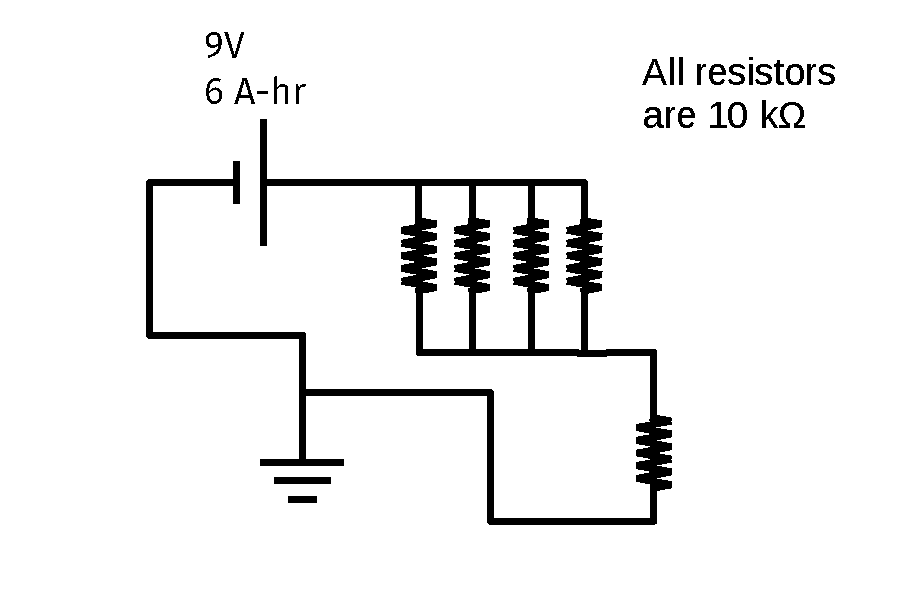
\includegraphics[width=0.5\textwidth]{figures/circuitExample5.pdf}
\caption{\label{fig:1}  A network of four resistors in parallel, all with $R = 10$k$\Omega$, in series with a fifth identical resistor.}
\end{figure}

\end{document}
